\section{Background} \label{sec:bg}


This section will provide a basic background information of history neuromorphic computing (\ref{sec:sb}) and the SpiNNaker (\ref{sec:sa}) in hardware architecture (\ref{sec:sa}) and software stack (\ref{sec:sss}). Then this section will explain some important conceptions in physics (\ref{sec:PB}) about the lattice Boltzmann method: why it is necessary and how it works. 


\subsection{History in a Nutshell} \label{sec:sb}
The vision of \textbf{neuromorphic computing}\cite{mead1980introduction} is to enable a new generation of computer architecture, designing energy-efficient general-purpose computing systems comparable to the human brain. In 1989, Carver Mead from Caltech first introduced the concept of \textit{neuromorphic Engineering} \cite{mead1980introduction}. From 1990 to 2003, the Von Neumann-based CPU industry continued to grow, Moore's Law \cite{schaller1997moore} was reaching its limits, and neuromorphic computing was dormant for more than a decade. In around 2004, the frequency growth of single-core processors slowed down, and IC designers turned to multi-core processors. Academia began to look for alternative technologies to the Von Neumann architecture.\\

In 2004, Kwabena Boahen from Stanford University developed Neurogrid \cite{benjamin2014neurogrid}, an analog circuit-based neural chip. In 2005, the University of Manchester began to develop \textbf{SpiNNaker}, a multicore neural supercomputer based on ARM chips. In the same year, the Europe, the US and IBM started their neuromorphic computing projects: FACETS project \cite{meier2004fast}, SyNAPSE project\cite{park2014impact} and Blue Brain project\cite{gara2005overview}, respectively. \\

In 2013, A 10-year-project, \textbf{Human Brain Project} began in 2013. It aims at building a research infrastructure to help advanced neuroscience, medicine, and computing \cite{hbp}. Although, the SpiNNaker project had started even before the Human Brain Project funded by the \textit{Engineering and Physical Sciences Research Council} (EPSRC), the Human Brain Project bring more funding and brilliant researchers building the 1 million core SpiNNaker machine since November 2018; see Fig~.\ref{fig:super_machine}.

\begin{figure}[!tb]
   \centering
       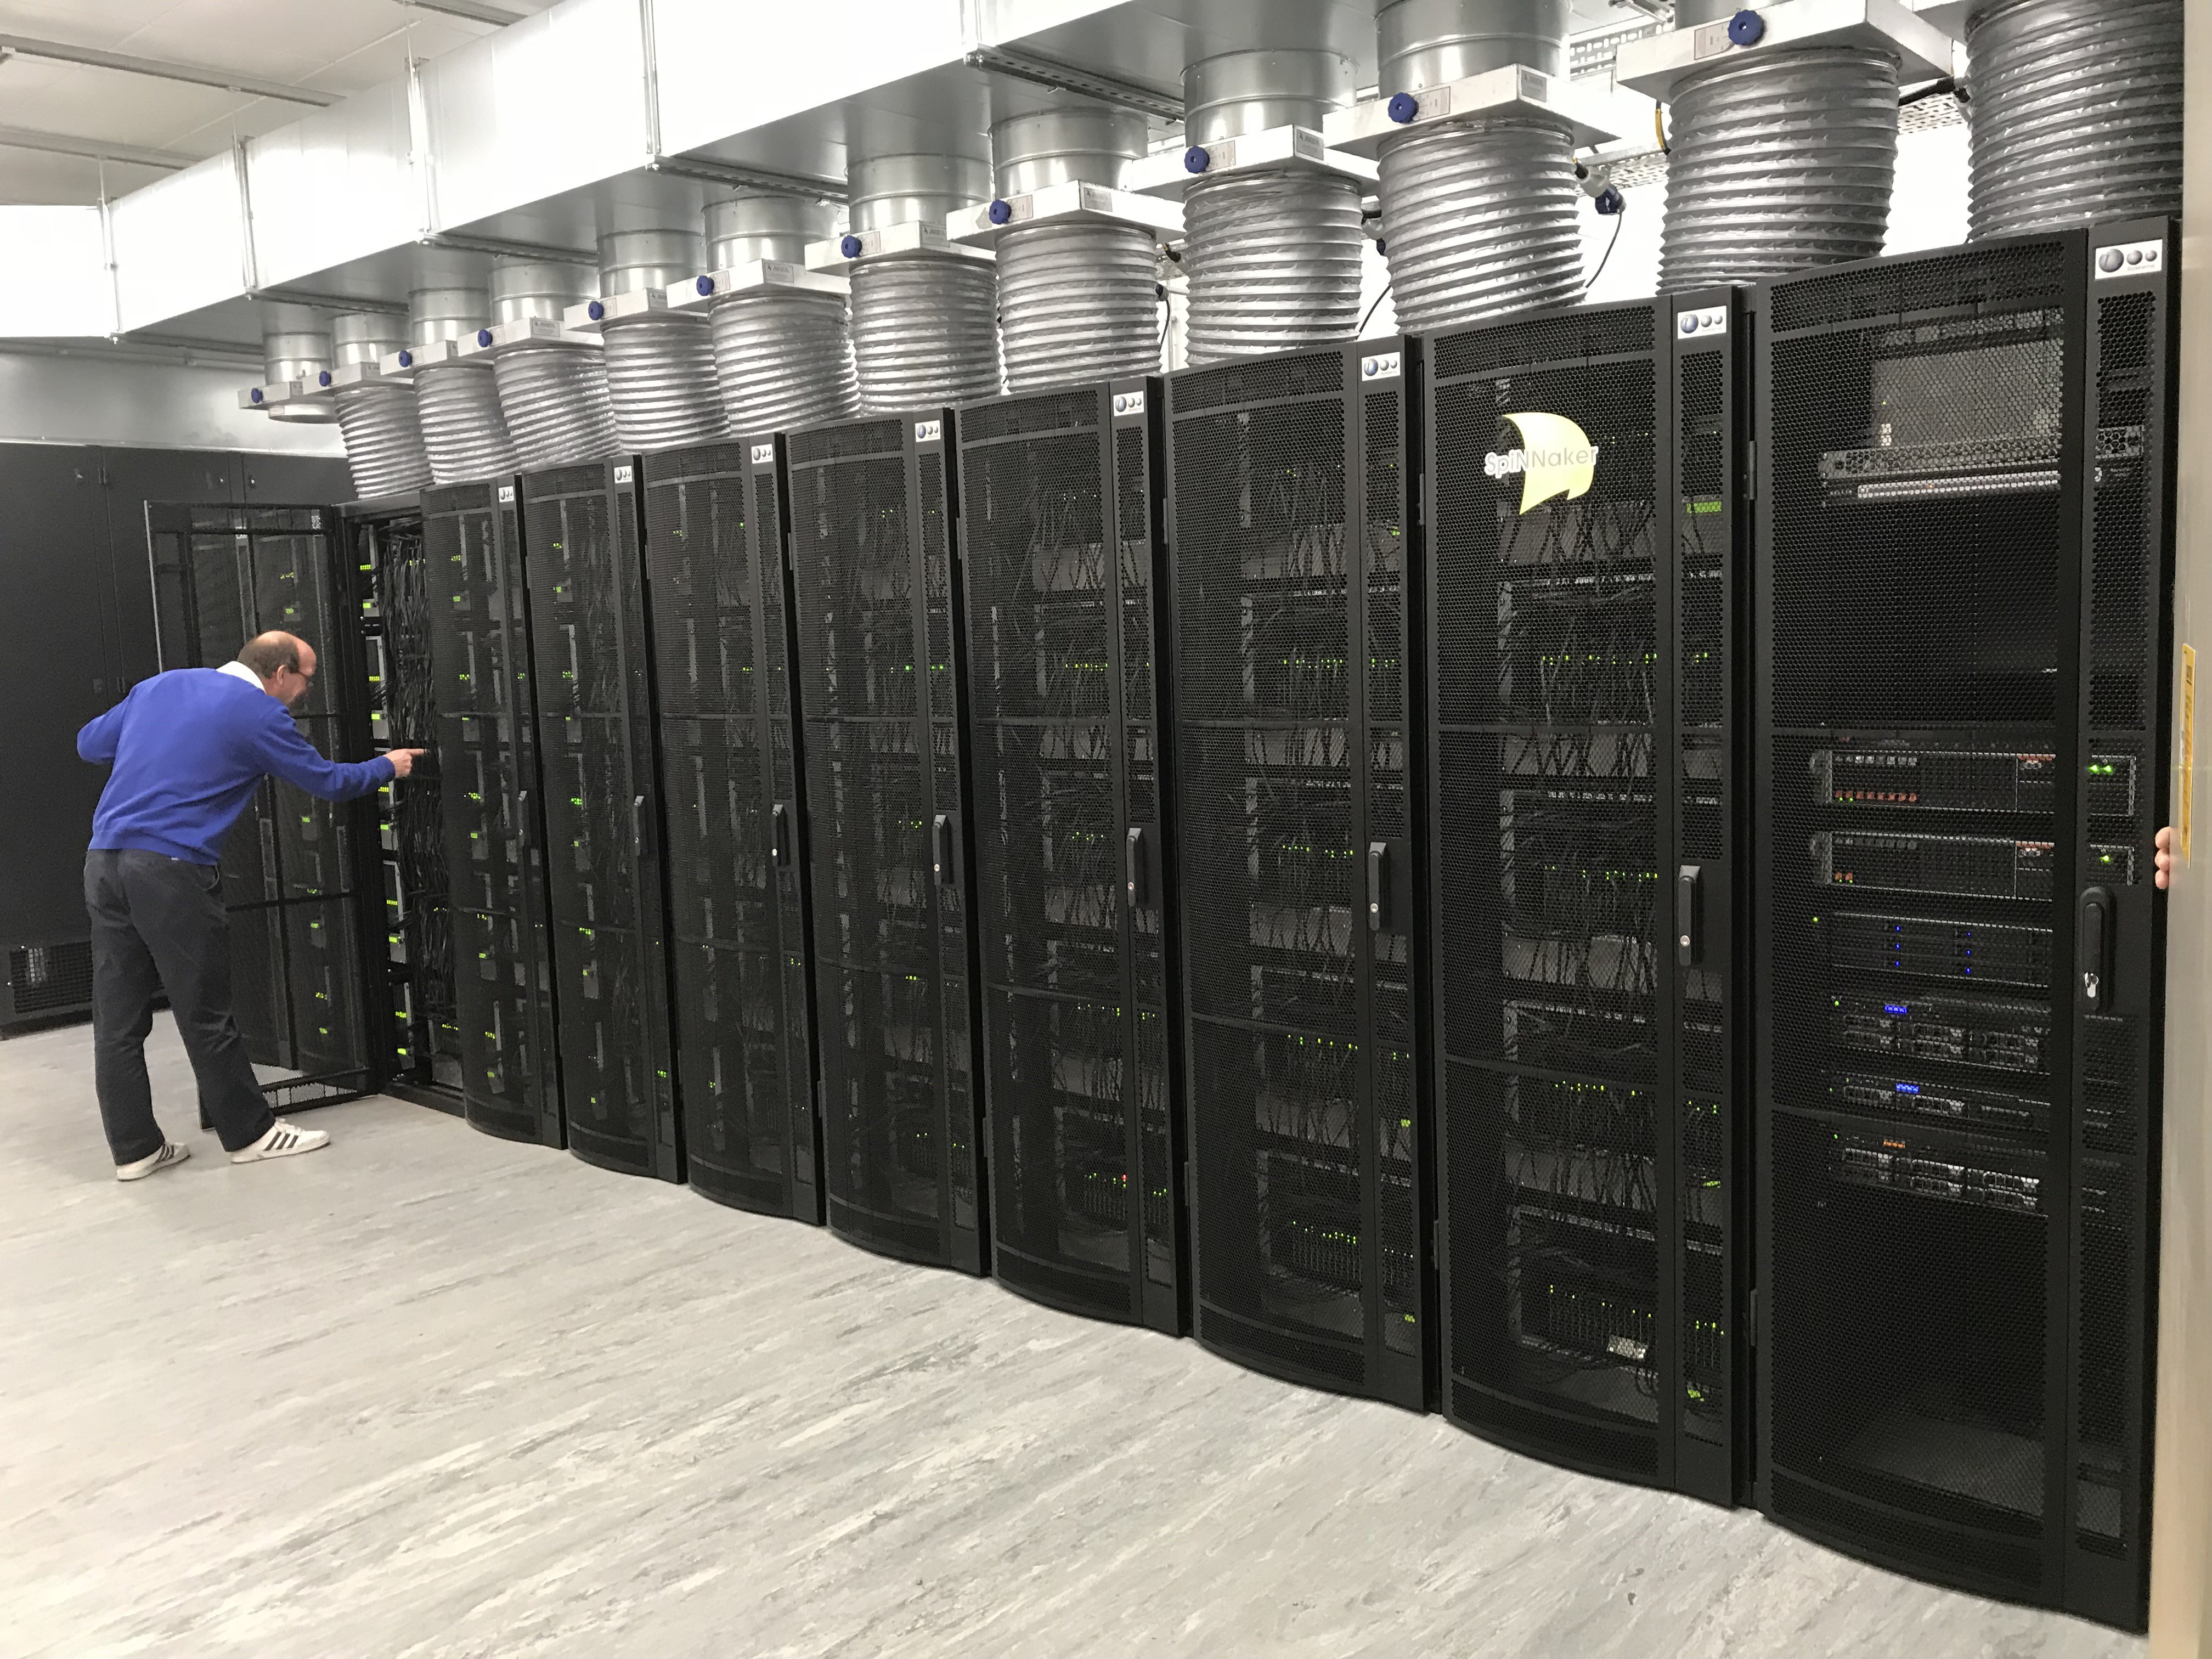
\includegraphics[width=0.8\textwidth]{figures/super_machine.jpg}
       \caption{Since November 2018: The 1 million core SpiNNaker HBP Platform machine((image from \cite{super_machine})).}
       \label{fig:super_machine}
\end{figure}



\subsection{SpiNNaker Architecture} \label{sec:sa}
In this subsection, we will illustrate the basic architecture of the SpiNNaker.
\subsubsection{Chip Architecture} \label{sec:ca}
\begin{figure}[!tb]
   \centering
       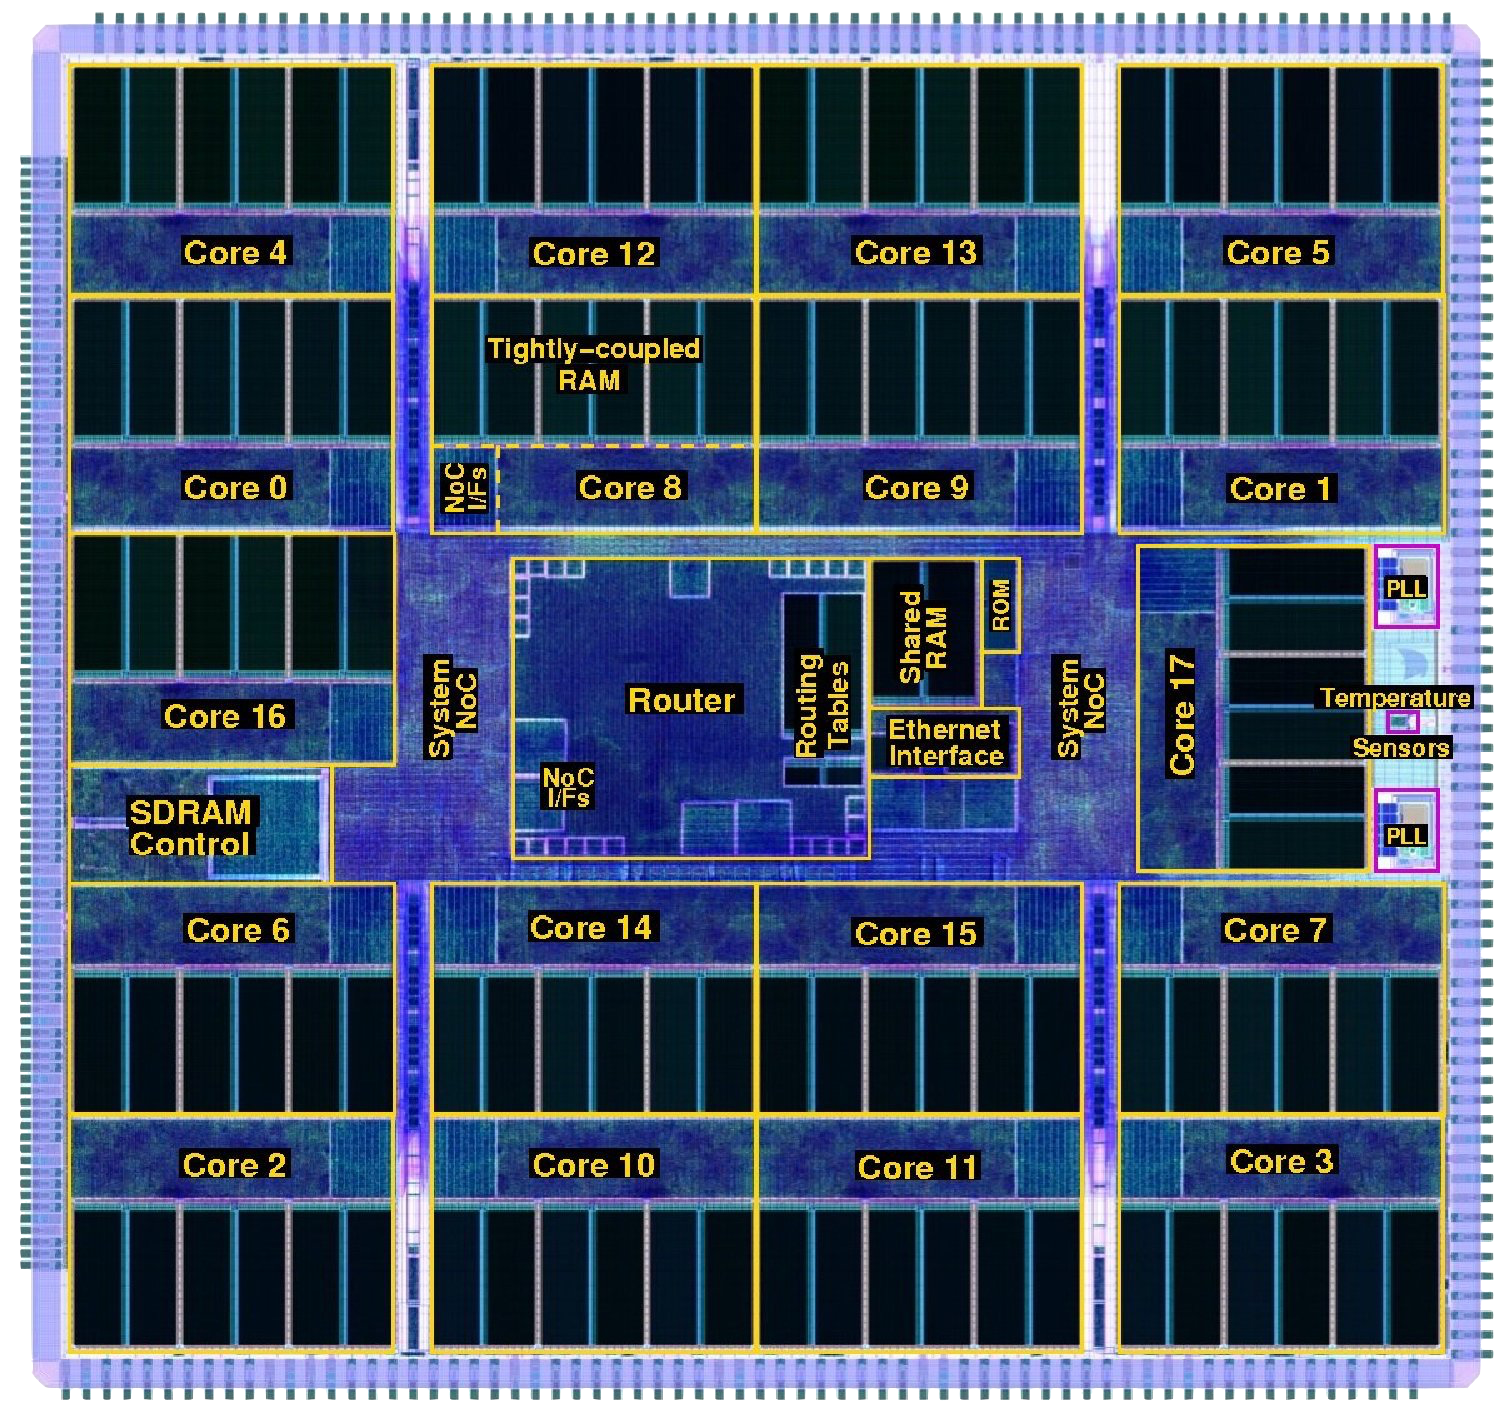
\includegraphics[width=0.8\textwidth]{figures/spinn_labeled_bw.png}
       \caption{An 18 cores SpiNNaker chip ((image from \cite{spinn-core})).}
       \label{fig:spinn-core}
\end{figure}
Fig.~\ref{fig:spinn-core} shows the die of a SpiNNaker chip that contains 18 cores. It mainly consists of \cite{furber2012overview}:

\begin{itemize}
    \item \textbf{ARM968 core:} Fig.~\ref{fig:spinn-core} . Being different from the most cores in the PCs or supercomputer running at $\sim GHz$, ARM968 is a medium-performance computing unit running at 200MHz with 220 DMIPS \cite{furber2012overview}. There are two very limited tightly coupled memory (TCM) blocks: a 64 Kbytes of data tight-coupled memory (DTCM) block and a 32 Kbytes of instruction tight-coupled memory (ITCM) block; see Fig.~\ref{fig:arm_968}. Other controllers including direct memory access (DMA) controller, communication controller, vectored interrupt controller are also built in. A major difference from the most cores in the market is that the ARM968 core do not have floating-point hardware and use fixed-point arithmetic instead. Though I might be more energy-efficient, it bring greater challenge to programmers \cite{furber2012overview}. Luckily, a software floating-point arithmetic is supported, though the performance might be slower and more memory-hungry \cite{spin-chip-resources}.
    \begin{figure}[!tb]
   \centering
       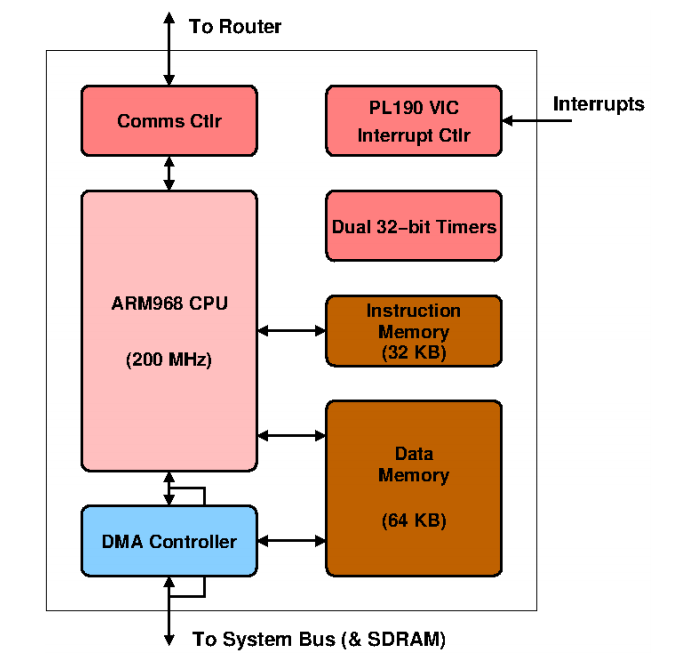
\includegraphics[width=1\textwidth]{figures/core.png}
       \caption{A diagram of SpiNNaker Core -- ARM 968 ((image from \cite{spin-chip-resources})).}
       \label{fig:arm_968}
    \end{figure}
    
    \item \textbf{Ethernet:} the SpiNNaker system connect to a host machine via Ethernet links \cite{furber2012overview}. Though an Ethernet MII (Media Independent Interface) is built-in each of the cores, only one core per board is using this interface. In term of speed, the Ethernet support around 10 Mbyte/s \cite{spin-chip-resources}. In type Spinn-5 board, there are extra three FPGAs (Field Programmable Gate Arrays) connected via SATA link which enable a higher bandwidth in this case. 
    
    \item \textbf{Router\label{sec:router}:} SpiNNaker cores communicate via passing message, where we call it "packet". When the SpiNNaker is running, there is a large number of packets going in and out each core, and, unlike the other message-passing framework in HPC, SpiNNaker cores send packets via a packet-switch network optimised for large numbers of small fixed-sized packets sent over the UDP/IP protocol. The Routers are responsible for put packets in and out. More communication details would be covered in Section \ref{sec:dt}.
    
    \item \textbf{System RAM:} When booting the machine, one of the core is elected to be a special processor as \textbf{Monitor Processor}. The rest cores are available for the application processing. For each chip, there is a 32Kbytes of System RAM used by either by the Monitor Processor when running neural network simulation or by all the cores when running non-neural simulation.
    
    \item \textbf{Sensors:} each SpiNNaker chip contains three temperature sensors, which are used to limit the clock rate when the temperature of chip rises too high.
\end{itemize}
\subsubsection{Network Topology}
Before we talk about how the SpiNNaker cores communicate, we need to illustrate how they are connected with its network topology.

In a SpiNNaker board, SpiNNaker chips are organized as a 2-dimension mesh network with bidirectional links to their six neighbours \cite{testchip}; see Fig.~\ref{fig:topology}. 

\begin{figure}[!tb]
   \centering
       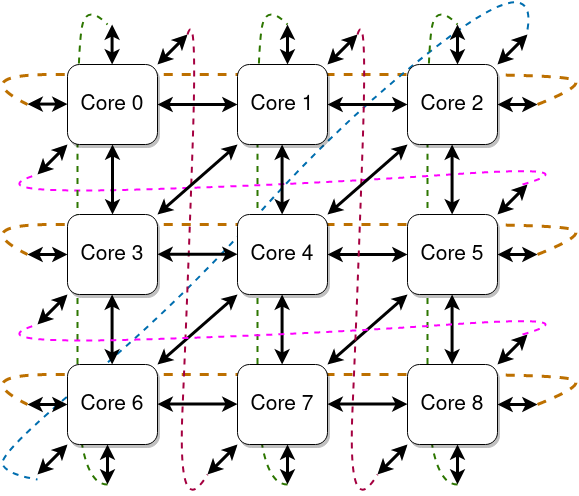
\includegraphics[width=0.8\textwidth]{figures/topology.png}
       \caption{The topology of nine SpiNNaker cores. Each core is connect with six other cores via bidirectional links. The cores on the boarder are connected with the core on the other end periodically.}
       \label{fig:topology}
\end{figure}

\subsubsection{Data Transmission in SpiNNaker} \label{sec:dt}
As we introduced before, SpiNNaker cores communicate with each other by passing message (packets). Each packet is of 40bits or 72bits (with a 32bits payload) \cite{furber2012overview} and there are four kinds\cite{ws6} of packet:

\begin{itemize}
    \item \textbf{Point-to-point (P2P) packet:} Point-to-point method is sending packets from a source core to a destination core. This method mainly used as system management.
    
    \item \textbf{Nearest-neighbour (NN) packet:} Nearest-neighbour method in SpiNNaker is unicasting or broadcasting data to neighbours i.e. six directly connected chips.
    
    \item \textbf{Fixed-route (FR) packet:} fixed-route method is sending packets from the SpiNNaker device to the host system. This method is mainly used as sending debugging data from a core back to the host machine.
    
    \item \textbf{Multicast (MC) packet:} Multicast is the primary communication format used by the SpiNNaker application developers and so does it in this project. With this method, the packets are sent once to multiple destinations; see Fig.~\ref{fig:multicast}  The routing key is allocated by the SpiNNaker system runtime. 
    
    As Fig.~\ref{fig:mc_pkt_layout} shows, a multicast packet contains an 8bits control header, a 32bits routing key and an optional 32bits payload. For every multicast router, it maintains a look-up table of routing masks and keys, and when a multicast packet come, it will compare the routing key with each entry in the look-up table. If it matches, the packet would be taken and it can also be sent to any other processors via the output links. In the case that the packet do not match with any entry in the look-up table, then the packets would be sent to the link opposite the input one which the packets arrived.
    
    It should be pointed out that in actual development the payload of the multicast packet should be in the format of 32bit integer. When the developer need to send a packet with payload in the other format, the developer need to union the payload into the format of 32bit integer.
\begin{figure}[!ht]
    \centering
    
    \begin{subfigure}[b]{0.9\textwidth}
    \centering
    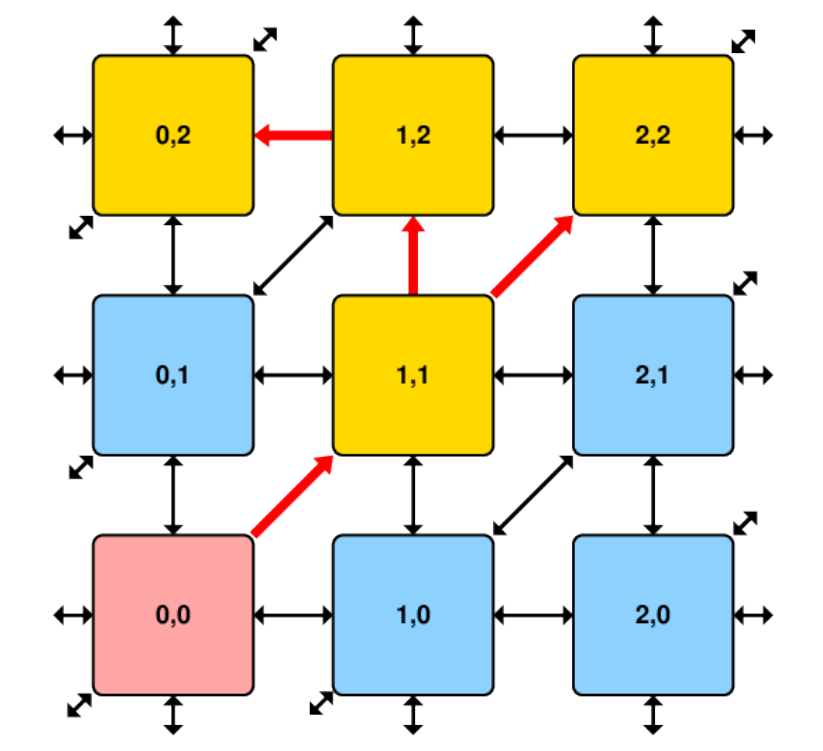
\includegraphics[width = 0.7\hsize]{figures/multicast.png}
    \caption{A Multicast show case, where core (0,0) send packet once to multiple destinations, core(1,1), core(1,2), core(0,1) and core(2,2).(image from \cite{ws6}).}
    \label{fig:multicast}
    \end{subfigure}
    ~
    \begin{subfigure}[b]{0.9\textwidth}
    \centering
    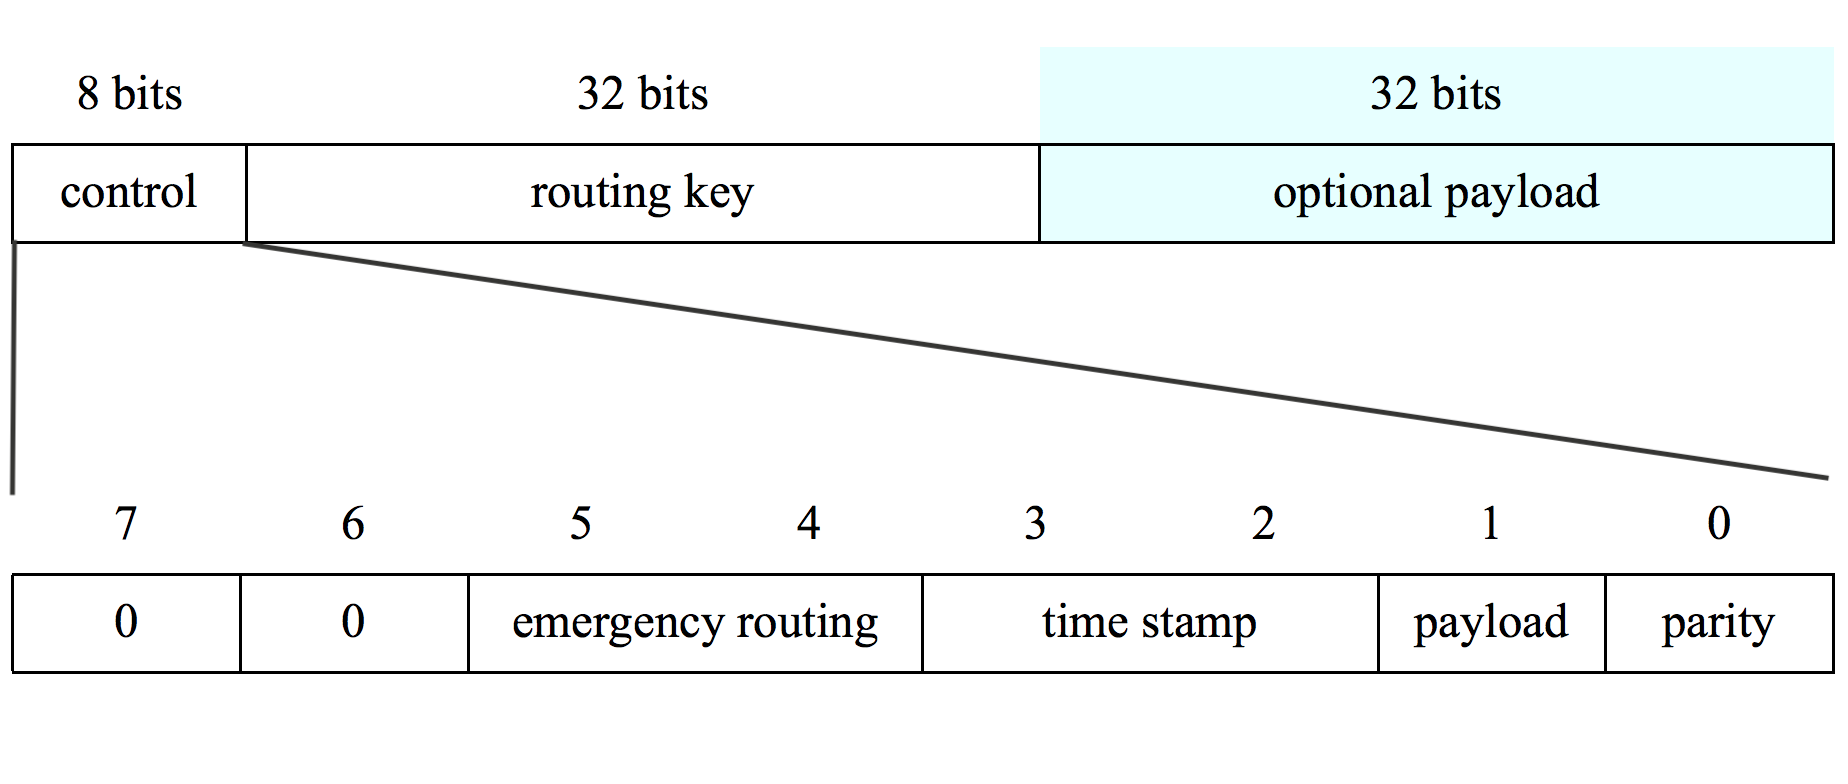
\includegraphics[width = 1\hsize]{figures/mc_pkt_layout.png}
    \caption{SpiNNaker Multicast Packet Space (image adapted from \cite{mc_pkt_layout}). A multicast packet contains an 8bits control header, a 32bits routing key and an optional 32bits payload. The multicast router use the routing key and a look-up table to match message it need.}
    \label{fig:mc_pkt_layout}
    \end{subfigure}
    \caption{How a packets is send via SpiNNaker multicast\ref{fig:multicast} and how is the memory space of a multicast packet\ref{fig:mc_pkt_layout}}
\end{figure}
\end{itemize}

As we discuss before, the SpiNNaker cores communicate over UDP/IP protocol. Thus \textbf{none of those four communication method guarantee the deliver of packets}, and as a consequence, the packets might be drop at any time. This situation may be exacerbated when there is a big amount of packets in the communication fabric. It is reasonable as in human brain, the spikes might be lost. However this characteristic brings difficulty for developing high-performance computing application, especially for those which are involved in huge message-passing. We will discuss the difficulty and solution at Section~\ref{sec:ssc}.

\subsection{SpiNNaker Application Development} \label{sec:sss}
\subsubsection{SpiNNaker Software Stack}
    \begin{figure}[!tb]
        \centering
       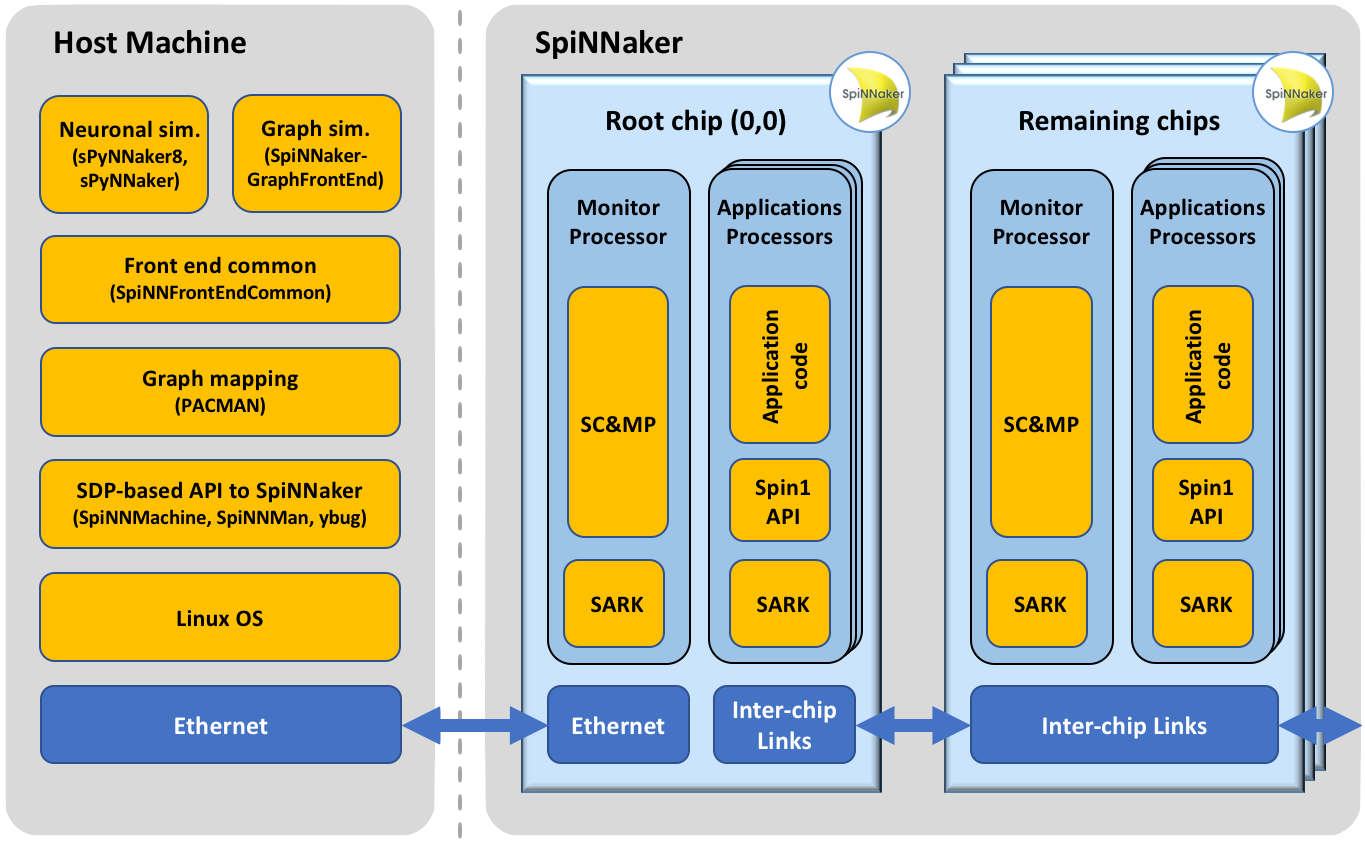
\includegraphics[width=1\textwidth]{figures/software_stack.png}
       \caption{A diagram of SpiNNaker Software Stack ((image from \cite{spin-chip-resources})).}
       \label{fig:software_stack}
    \end{figure}

Fig.~\ref{fig:software_stack} shows what SpiNNaker software contains and how it works. High-level abstractions for Neural simulation (\textit{sPyNNaker}) and general parallel computing (\textit{SpiNNaker GraphFrontEnd}) provide APIs for developers to describe the neural connection or computational graph. Since we are not developing neural simulation application, the primary software we used for this project is the SpiNNaker GraphFrontEnd. 

After the computational graph is described by the developers in Python, the Partition and Configuration Manager system (\textit{PACMAN}) will map the computational graph to the SpiNNaker cores. 

The actual computation of each vertex is defined via the \textit{Spin1} API in C code. Both of the partition information and the pre-compiled computation job are transferred to the root chip of SpiNNaker machine via Ethernet. Then the information would be passed to the rest of the chip in the board via  the inter-chip connection.


Sitting on the lowest layer of the software stack, the SpiNNaker application runtime kernel (\textit{SARK}) support the runtime system of the SpiNNaker core. 


\subsubsection{SpiNNaker Development Workflow} \label{sec:sdw}

For this project, instead of neural simulation, we are using the SpiNNaker as a parallel computer and our workflow of development are using the GraphFrontEnd API.

Firstly, even before we define the computation of each individual vertex, we need to define the data specification information such as what data we are going to pass to the SpiNNaker, how many router keys does a vertex may want via the \textit{SpiNNFrontEndCommon} and \textit{PACMAN} API. After we define our vertex, we need to define the edge between the vertex via \textit{PACMAN} API.

Then we need to express our communication fabric as a graph by connecting the vertices together with the edge we just defined via the \textit{SpiNNaker GraphFrontEnd} API in Python. 

After we got our computational graph, we then need to define the computation and communication of each individual vertex in C via the \textit{Spin1} and \textit{simulation} APIs, etc.

\subsection{Development Environment for SpiNNaker} \label{sec:impl}
At the beginning of this project, our first choice to access the SpiNNaker machine is to use a directed connected broad for development. However, later on, there is problem with the connection port. Due to the pandemic COVID-19, the repair is not available. We then switch to the web interface with the Jupyter Notebook. There are many ways to get access to the SpiNNaker machine, we will mainly discuss those two method that are used during this project.
\subsubsection{Directed Connected Board with IDE}
The first choice for this project is to run the simulation with physically board connecting with the laptop. As shown in the Fig.~\ref{fig:laptop}, SpiNNaker developers can make all the development offline. Typically, they write code in their host computer with a code editor or an IDE then offload the simulation to the connected SpiNNaker board.\\

One of the advantages of development with a SpiNNaker Board is that the developers can physically watch the running condition of the SpiNNaker boards and make corresponding manipulation. Another advantage is that the developers can make full use of their favourite code editors or IDEs, which makes it easier to view the source code and debugging.\\

There are some disadvantages though. A major disadvantage is that it is the developers' duty to maintain the development condition of the SpiNNaker board including the Ethernet connection, electronic power and the condition of the SpiNNaker board itself. Most SpiNNaker users are not professional electronic engineers, so if there is any trouble with those problem, the developers must try to get help from the SpiNNaker team or they are on their own. \\

\begin{figure}
\centering
   \centering
       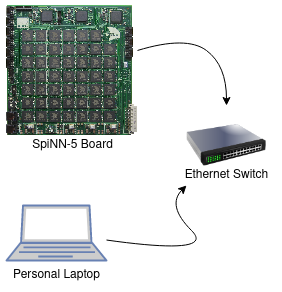
\includegraphics[width=0.8\textwidth]{figures/laptop.png}
       \caption{Development with Directed Connected Board via Ethernet switch ( board image from \cite{spinn-core}). Developers need a physical board, but they can use their desirable development environment.}
       \label{fig:laptop}
\end{figure}


\subsubsection{Web interface with Jupyter Notebook}
For most SpiNNaker users or who are just get into the SpiNNaker development, they may not even have a board. The best way to write SpiNNaker to develop SpiNNaker application is using the web interface development by the SpiNNaker team. \\

With the web interface, the developers run the python code within the Jupyter Notebook. The Jupyter also provides a terminal enabling the developers compile their C code and run shell command. For this project, we compile the C code on the laptop and upload the binaries to the remote system and run the application in the Jupyter notebook(shown in Fig.~\ref{fig:jupyter}).\\

The biggest advantage of developing with the Jupyter interface is that the developers do not need to take extra concern on the board maintain. They can pay full attention on the application development even if they do not even have a board. Another advantage is that there are more than 1 million cores available remotely. They developer can scale their application up with the Jupyter notebook easily. Though it might be easier for developer to connect with a SpiNNaker machine via the Jupyter, it is hard to view the source code of the APIs and debugging in the Jupyter. \\

Overall, for hardcore developers or absolute beginners, it might be better to use the connected board to develop SpiNNaker framework or applications and getting familiar with the SpiNNaker API stack. For those who have been already familiar with the SpiNNaker API stack and want to scale their application up, it might be better to use the Jupyter interface.\\

For this project, our first choice was using a directed connected Spinn-5 board and an IDE on the laptop. Later on, in the second half of this research, the connection between the board and the laptop started to become unstable. We then decided to switch to the Jupyter interface.\\

\begin{figure}[!tb]
\centering
    \centering
   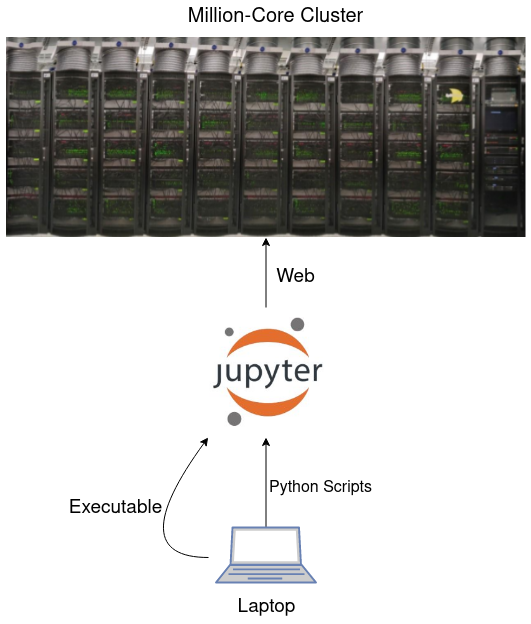
\includegraphics[width=0.8\textwidth]{figures/jupyter.png}
       \caption{Development with Jupyter Web interface ( board image from \cite{spinn-core}). The SpiNNaker team has maintain the environment and user can development directly in Notebook, but with less customized environment and less convenient debugging experience.}
       \label{fig:jupyter}
\end{figure}


\subsection{Physics Background} \label{sec:PB}
% KS: Need to clearly separate what is the kinetic theory of gases and the Boltzmann
% equation, and what is lattice Boltzmann. REFERENCES?

% KS: What are the Navier Stokes equations?
\subsubsection{Fluid Model in Brief}
Fluids are physically discrete systems composed of a large number ($~10^{23}$) of particles \cite{lbmmbook}, where every particle is constantly doing Brownian motion and exchange momentum and energy by collision. Thus the microscopic structure and motion are quite complex in both space and time. On the other hand, contrary to the inhomogeneity, dispersion, and randomness of microscopic motion, the macroscopic motion of the fluid exhibits uniformity, continuity, and determinism. The macroscopic motion and other properties of the fluid are the result of averaging the microscopic motions of the fluid molecules. Therefore, the mathematical models describing fluid motion can vary considerably when observed at different scales.\\

In general, methods for describing fluid systems can be classified into Molecular Dynamics model, Mesoscopic Model and macroscopic continuum models depending on the scale; see Fig.~\ref{fig:fluid_models}. The Molecular Dynamics model views the fluid as a many-body system consisting of a large number of molecules and focuses on the dynamic behavior of each fluid molecule (at \ref{sec:HE}). Through the movement of each molecule of the statistical representation to describe the overall motion of the fluid; macroscopic continuum model of the fluid as a continuous whole, focusing on the fluid microscopic group, with a set of partial differential equations (Navier Stokes Equations \ref{sec:nse}) to describe the macroscopic motion of the fluid; mesoscopic dynamic model, including the lattice Boltzmann model, focuses on the velocity distribution function of the fluid molecules, by expressing its macroscopic physical quantities and distribution function over time to obtain macroscopic flow Information (Boltzmann Equation \ref{sec:BE}). \\

\begin{figure}[!tb]
   \centering
       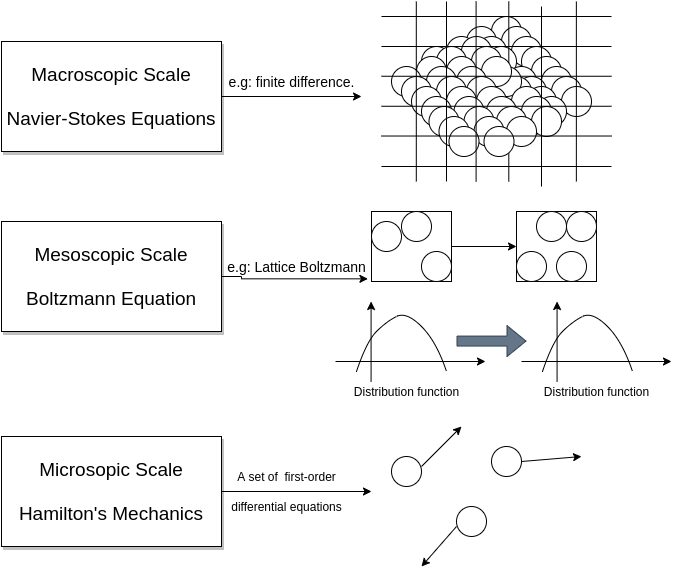
\includegraphics[width=1\textwidth]{figures/comparsion.png}
       \caption{Three different kinds of fluid models.The one on the top represent macroscopic models, including finite difference, finite element, etc, which mainly apply the Navier-Stokes Equations. The one in the middle represent mesoscopic models, such as LBM. Those models apply Boltzmann Equation. The bottom one represent microscopic models, which apply Hamilton's mechanics/equations. }
       \label{fig:fluid_models}
\end{figure}

The lattice Boltzmann method (LBM) as a mesoscopic model set in the between the microscopic model and the continuum model. It enjoy the advantages of both the macroscopic and microscopic approaches, and we will introduce both of them next before the LBM.

\subsubsection{Navier-Stokes Equations -- Macroscopic Model} \label{sec:nse}
In general, a fluid can be viewed as a continuous medium that fills the entire flow field, so that the physical quantities of density, velocity, temperature, etc. can be defined at each point of the flow field and a series of partial differential equations can be established to describe the motion of the fluid. The continuous medium assumption is a fundamental assumption of fluid mechanics and is an approximate treatment of macroscopic fluid structure.\\

Based on the assumption of a continuous medium, the motion of a fluid follows the law of conservation of mass, momentum and energy, which can be mathematically described by a set of partial differential equations Equation.~\ref{equ:NS}:

\begin{equation}
    \left\{\begin{matrix}
\frac{\partial \rho}{\partial t} + \triangledown \cdot (\rho u) = 0\\ 
\\
\frac{\partial (\rho u)}{\partial t} + \triangledown \cdot (\rho u u) = 0\\ 
\\
\frac{\partial (\rho u)}{\partial (t) + \triangledown \cdot (\rho u e)} = \sigma : \triangledown u - \triangledown \cdot q
\end{matrix}\right.
\label{equ:NS}
\end{equation}

Here in Equation ~\ref{equ:NS}, $\rho$, $u$, $T$ and $e$ are the density, speed, temperature and internal energy per unit mass, respectively. $\sigma$ is the strain tensor and $q$ is the heat flux from heat transfer and heat radiation.

The Equation ~\ref{equ:NS} is not in closed-form. In order to obtain the complete equations, the equations of states need to be supplemented with the relationship between the stress tensor and the rate of deformation tensor, between the heat flow vector and the temperature gradient, and with the thermodynamic properties of the associated thermodynamic properties. For Newtonian fluids, the stress tensor is linearly related to the deformation rate tensor and can be expressed as, where $I$ is the second-order unit tensor, $p$ is the static pressure, $\tau = 2 \mu S + \lambda(\triangledown \cdot u)I$ is the viscous stress tensor, where $\mu$ is the dynamic viscosity coefficient, $\lambda$ is the second viscosity coefficient, and $S$ is the deformation coefficient tensor, which is defined as Equation~\ref{equ:DCT}:

\begin{equation}
    \label{equ:DCT}
        S_{a b} = \frac{1}{2} (\frac{\partial u_a}{\partial x_b} + \frac{\partial u_b}{\partial x_a})
\end{equation}

Under the Stokes' hypothesis \cite{gad1995stokes}, the two types of viscosity coefficients are related by: $\lambda + (2/3)\mu = 0$. By applying the Stokes' hypothesis, the Equation ~\ref{equ:NS} can be called Navier-Stokes equations. \\

In this project, we do not need to consider the temperature (T), energy (e) or heat flux (q). In this case, the system need to meet the conservation of mass and momentum; see Equation~\ref{equ:conservation} and $f$ is the force on the fluid. 

\begin{equation}
    \label{equ:conservation}
        \begin{matrix}
        \frac{\partial \rho}{ \partial t} + \nabla (\rho u) = 0 \\
        \frac{\partial{\rho u}}{\partial t} + \nabla \cdot (\rho u u ) = f \\
        \end{matrix}
\end{equation}

The external force $f$ can be written as Equation~\ref{equ:force}, where $p$ in the isotropic pressure and $\tau$ is a stress.
\begin{equation}
    \label{equ:force}
    f = -\nabla p + \nabla \cdot \tau
\end{equation}

Correspondingly, according to the Stokes assumption, the stress $\tau$ can be written as Equation~\ref{equ:stks}, where $\eta$ is the dynamic viscosity which describes, at a macroscopic
scale, the effect of collisional diffusion of momentum between molecules. 
\begin{equation}
    \label{equ:stks}
    \tau_{ab} = \eta (\frac{\partial u_a}{ \partial x_b} + \frac{\partial u_b}{\partial x_b})
\end{equation}


\subsubsection{Molecular Dynamics model -- Microscopic Model} \label{sec:HE}
The continuum models with Navier-Stokes equations do not take into account the microscopic molecular model of the fluid and directly describes the macroscopic physical quantities of the fluid, but the fluid is physically composed of fluid molecules, and the macroscopic motion of the fluid is the result of averaging the thermal motion of the microscopic molecules. Therefore, if the microscopic motion of the fluid molecules can be known, the macroscopic physical quantities of the fluid can theoretically be obtained by averaging. This is the basic idea of the molecular dynamics model. The molecular dynamics model looks at the microscopic molecular motion of a fluid, studies the time evolution of the spatial position and velocity of the fluid molecules, etc., and uses statistical methods to obtain information on the macroscopic flow from the microscopic information of the molecules.\\

In general, Hamiltonian equations are applied to this model \cite{salmon1988hamiltonian}, but the reasoning is beyond the scope of this project. With the idea of describing the macroscopic physical quantities by averaging the microscopic particles, we can then move to the kinetic theory of gas.

\subsubsection{Kinetic Theory of Gas}\label{sec:BE}
Kinetic theory is the branch of statistical physics dealing with the dynamics of non-equilibrium process and their relaxation to thermodynamic equilibrium \cite{succi2001lattice}. The theory of gas kinetics is based on the molecular model, which holds that a gas is made up of a large number of molecules ($10^{23}$) and that the molecules are always in constant random motion. The interaction between any two molecules can be expressed as a function of distance, such as the simplest molecular model of a rigid sphere model, which holds that two molecules interact only when they are in contact, and the inter-molecular interaction function is Equation~\ref{equ:hard_sphere}:\\

\begin{equation}
\label{equ:hard_sphere}
\phi  (r) = \left\{\begin{matrix}
\infty, & r \leqslant \sigma \\ 
0, & r > \sigma
\end{matrix}\right.
\end{equation}

Here, $r$ is the distance between two molecular and $\sigma$ is the diameter of molecular.\\

However, for gas systems consisting of a huge number of molecules ($10^{23}$), tracking the motion of each molecule based on the forces between molecules as in molecular dynamics is impractical for most systems. Applying statistical methods to study the statistical characteristics of these discrete molecules, such as the average number of molecules in a small volume unit and over small time intervals, the average velocity, the average energy, and other relevant physical quantities, is a feasible approach, and this is the fundamental point for kinetic theory of gas and the Boltzmann Equation.

\subsubsection{Boltzmann Equation -- Mesoscopic Model}
Ludwig Eduard Boltzmann (1844-1906), the Austrian physicist explains and predicts how the properties of atoms and molecules (microscopic properties) determine the phenomenological (macroscopic) properties of mater including viscosity, thermal conductivity\cite{lbmmbook}. He proposed and developed the Boltzmann equation, which then become the starting point of the kinetic theory of gas.\\

To describe the Boltzmann equation, in any macroscopic system, the microscopic motion of each molecule follows the laws of mechanics, so as long as the individual motion of a large number of particles, you can determine the macroscopic parameters of the whole system, which is the basic starting point of molecular dynamics; from another perspective, instead of determining the state of motion of each molecule, we can find the probability of each molecule in a certain state, which can be obtained by statistical methods. This is the basic idea behind the Boltzmann equation, which is the equation used in statistical mechanics to express the evolution of an non-equilibrium distributed function; see Equation ~\ref{equ:BE}.

\begin{equation}
\label{equ:BE}
    \frac {\partial f}{\partial t} + \vec u \cdot \triangledown _x f + \vec a \cdot \triangle _ u f = \Omega (f)
\end{equation}

In Equation ~\ref{equ:BE}, $f$ is the velocity distribution function; $u$($u_x$,$u_y$,$u_z$,) is the the molecular velocity vector; $t$ is the time; $a$ is the acceleration (given by the external force $F=ma$); $\Omega$ is the collision operator or collision term \cite{succi2001lattice}.

The Boltzmann equation (Equation~\ref{equ:BE}) is a complex integro–differential equation. It is unrealistic to get an exact solution. In this case, lattice method become a feasible way to compute and model the fluid. Lattice Gas Automata (LGA) \cite{frisch1986lattice} is one of them; and the lattice Boltzmann method derived from it.

But before introduce the lattice Boltzmann method, we need to talk about another important concept, Bhatnagar-Gross-Krook Collision (\ref{sec:BKG}).

\subsubsection{Bhatnagar-Gross-Krook approximation} \label{sec:BKG}
Because of the close relationship between the Boltzmann equation and the fundamental equations of fluid mechanics, the Boltzmann equation could be solved numerically to simulate the macroscopic motion of a fluid. However, since it is not practical to solve Boltzmann equation directly, the biggest difficulty lies in its collision term\cite{chew1956boltzmann}. Therefore, it is a natural idea to use a simple form of collision instead of the collision term, and the Bhatnagar-Gross-Krook (BGK) approximation/collision \cite{bgk} arises in this context.

BGK approximation was firstly proposed by Bhatnagar, Gross and Krook in 1954 \cite{bgk}. They think that a collision term should: 

\begin{itemize}
\item \textbf{Satisfy the conservation of mass, momentum and energy}. 

\item \textbf{Be able to reflect the tendency of the system towards equilibrium}
\end{itemize}

A simple collision term can draw from those two assumption with assuming the effect of a collision is to change the distribution function $f$ so that it tends to an equilibrium distribution $f^{eq}$. Set the rate of change to be proportional to the difference between $f$ and $f^{eq}$, and $\tau$ is the relaxation time. So you can introduce a BGK collision term $\Omega (f)$ at Equation ~\ref{equ:BGKLB}:

\begin{equation}
\label{equ:BGKLB}
    \Omega (f) = \tau(f_{eq} - f)
\end{equation}

Equation~\ref{equ:BGKLB} is called Boltzmann\_BGK equation \cite{chew1956boltzmann}. The BGK approximation greatly simplifies the solution of the equation.

\subsubsection{Lattice Boltzmann Method in Brief} \label{sec:lbmb}
The basic idea of the lattice Boltzmann is imagine the fluids including gases as a great number of particles that are moving with random states. The particles exchange their momentum and energy by streaming and collision. We can describe the process as the Boltzmann transport equation Equation ~\ref{equ:BTE}:
\begin{equation}
\label{equ:BTE}
    \frac{\partial f}{\partial t} + \vec{u}\cdot \nabla f = \Omega
\end{equation}
In Equation~\ref{equ:BTE}, $f(\vec{x}, t)$ is the distribution function, $\vec{u}$ is the velocity of particles and $\Omega$ represent the collision term. In this project, the lattice would be simplified to be in two dimensions. The velocities $\vec{u}$ are described as \textit{macroscopic velocities}, whilst in this project the there would be 9 \textit{microscopic velocities} (seen in Fig.~\ref{fig:d2q9} and labelled as $\vec{e}_1...\vec{e}_9$). 

In 1992, Qian et al. \cite{d2q9} proposed DdQm ($d$ dimensions, $m$ discrete velocities) models, which are the basic models of LBM. Fig.~\ref{fig:d2q9} shows a D2Q9 model and its nine discrete velocities in two dimensions. Correspondingly, in Equation.~\ref{equ:d2q9}, we introduce the discrete velocities $e_i$ in two dimensions.

% KS: I would try to put Figures either at the top or the bottom
% of the page so they don't interupt the text, so use tb in the
% command for figure. Figures should be 'called out' in the text
% so put a label in the figure and reference it in the text.


\begin{figure}[!tb]
   \centering
       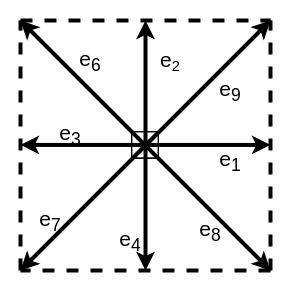
\includegraphics[width=0.5\textwidth]{figures/nine_direction.jpg}
       \caption{A lattice in D2Q9 model and its nine discrete velocities}
       \label{fig:d2q9}
\end{figure}

\begin{equation}
\label{equ:d2q9}
    \vec{e}_{i} = \left\{\begin{matrix}
(0,0) \qquad\qquad\qquad\qquad\qquad\qquad &i=0 \\ 
(1,0), (0,1), (-1,0), (0,-1)\quad\qquad &i=1,2,3,4 \\ 
(1,1), (-1,1), (-1,-1), (1,1)\qquad & i=5,6,7,8
\end{matrix}\right.
\end{equation}

For each lattice, the distribution function can be thought of as a measure of the probability that the fluid at given position $\mathbf{x}$ has velocity $\mathbf{e}_i$ at time $t$.

As introduced above, in lattice Boltzmann method, the behaviour has been described as the streaming and collision step which are given by Equation~\ref{equ:lbmequ}. In this equation, $fi$ is the distribution function in the direction i; $\tau$ is the relaxation time; $f_i^{eq}$ is the equilibrium distribution function in the direction i; $t$ and $\triangle t$ is the time and the increment of time.

\begin{equation}
\label{equ:lbmequ}
f_i(\vec{x}+c\vec{e_i}\triangle t, t+\triangle t) - f_i(\vec x,t)) = \frac{f_i(\vec x, t) - f_i^{eq}(\vec x , t)}{\tau}
\end{equation}



% KS: EXPLAIN ALL SYMBOLS WHEN THEY ARE FIRST INTRODUCED!

In Equation~\ref{equ:lbmequ}, in the left of the equal sign stand for the streaming step and the collision step is in the right. In the actual implementation of our lattice Boltzmann method, we will calculate them separately. The Fig.~\ref{fig:stream} shows how the streaming step exchange its discrete probability distribution.


\begin{figure}[!tb]
   \centering
       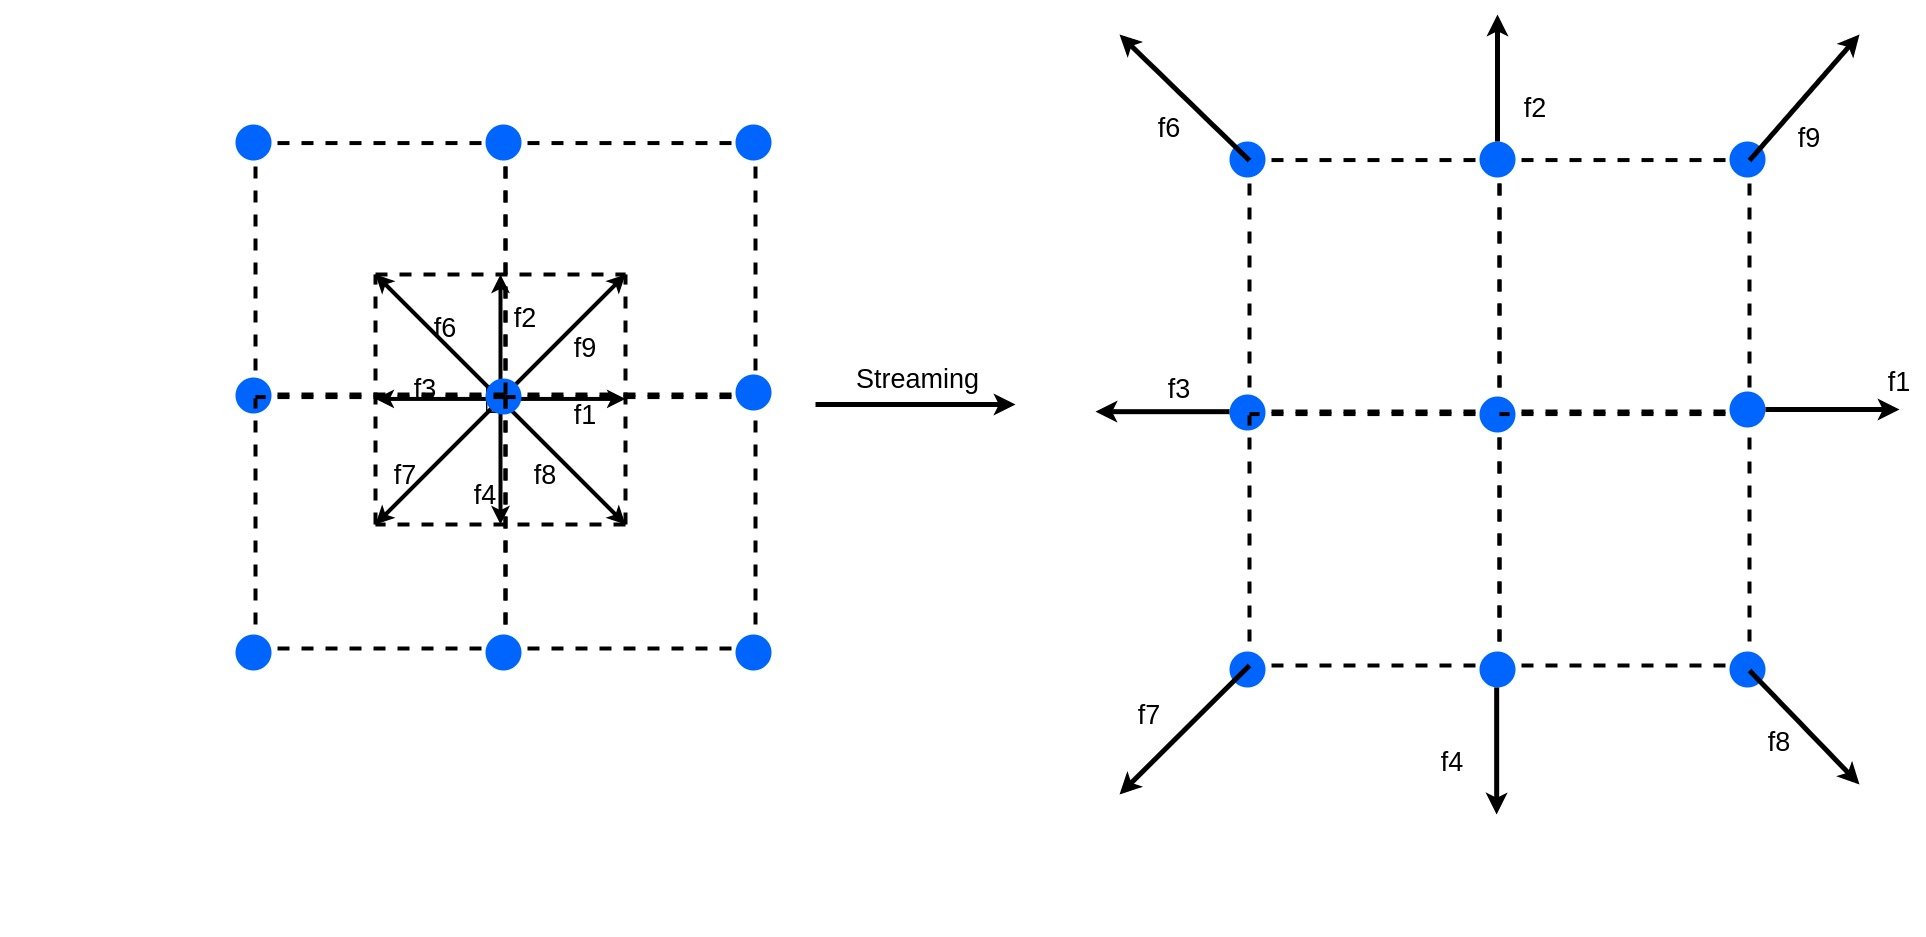
\includegraphics[width=1\textwidth]{figures/stream.jpg}
       \caption{The streaming step of a lattice in D2Q9 model}
       \label{fig:stream}
\end{figure}

In the collision step, Bhatnagar-Gross-Krook (BGK)\ref{sec:BKG} approximation is applied to model the process of relaxation to equilibrium. Qian et al represent the equilibrium distribution function in their the DdQm models as Equation~\ref{equ:collision}. Macroscopic density $\rho$, velocity $u$, weighting factor $\vec{\omega_i}$ and lattice speed $c$ are introduced to this process in Equation~\ref{equ:collision}:

\begin{equation}
\label{equ:collision}
    f_i^{eq}(\vec x, t) = \vec{\omega_i} \rho + \rho \vec{\omega_i} \left [  \frac{\vec{e_i}\cdot \vec u}{c^2} + \frac{(\vec{e_i}\cdot\vec u)^2 }{ 2 \cdot c^4 }-\frac{\vec u \cdot \vec u}{2 \cdot c^2} \right ]
\end{equation}

According to Qian et al.'s model of D2Q9, $\omega_i$ is given as:
\begin{equation}
    \vec{\omega_i} = \left\{\begin{matrix}
4/9 & i=0\\ 
1/9&\quad \quad i=1,2,3,4\\ 
1/36&\quad \quad i=5,6,7,8 
\end{matrix}\right.
\end{equation}

Macroscopic fluid density $\rho (\vec x, t)$ is defined in this model by Equation~\ref{equ:rho}:
\begin{equation}
\label{equ:rho}
    \rho (\vec x, t) = \sum_{i=0}^{8} f_i(\vec x,t)
\end{equation}

Macroscopic velocity $\vec u(\vec x, t)$ is defined in this model by Equation~\ref{equ:u}:
\begin{equation}
\label{equ:u}
    \vec u (\vec x, t) = \frac{1}{\rho} \sum_{i=0}^{8}cf_i\vec{e_i}
\end{equation}

After all, we can summarize the algorithm as follow:
\begin{itemize}
  \item [1] Initialize macroscopic fluid density$\rho$, macroscopic velocity $\vec u$, and discrete probability distribution function $f_i^{eq}$;
  \item [2] Compute the $\rho$, $\vec u$ with Equation~\ref{equ:rho} and Equation~\ref{equ:u};
  \item [3] Compute the equilibrium distribution $f^{eq}_i$ with Equation~\ref{equ:collision};
  \item [4] Collision Step: Update the distribution function $f_i$;
  \item [5] Streaming Step: move $f_i$ to the $f_i^*$ in all nine direction with regarding to $\vec{e_i}$
\end{itemize}


With different initial parameters, the lattice Boltzmann method can simulation different physical problem. As we have discussed in \ref{sec:Obj}, Minion and Brown's problem\cite{minion1997performance} was chosen as a test problem. We will now discuss how to set the initial parameters to assure we are discuss a same physical problem.

% KS: WHAT INITIAL PARAMETERS DO YOU HAVE? 

\subsection{Initial Parameter}
To assure that the implementation is simulating the Minion and Brown's problem\cite{minion1997performance}, we need a criteria. In this case, the Reynolds number can be the criteria. The Reynolds number is the ratio of inertial forces to viscous forces within a fluid which is subjected to relative internal movement due to different fluid velocities\cite{munson2013fluid}. It is used to measure the similitude between fluid dynamics. If we set our parameters to have the same Reynolds number as the case in Minion and Brown's problem, we can assure that we are simulating their problem. In the definition of the Reynolds number at Equation~\ref{equ:neynolds}, $U$ is the velocity, $L$ the length scale, and $\nu$ is the kinematic viscosity.
\begin{equation}
\label{equ:neynolds}
    Re = \frac{U \cdot L}{\nu}
\end{equation}

In the Minion and Brown's problem, the initial velocity $u$ is defined as Equation~\ref{equ:init_u}, where $k$ is the shear layer thickness; $x$ and $y$ are the position in the system ; $\delta$ is a velocity. 

\begin{equation}
\label{equ:init_u}
    \begin{matrix}
u = tanh(k (y-0.25)) & y \leqslant 0.5 \\ 
u = tanh(k (0.75-y)) & y > 0.5  \\
v = \delta sin(2\pi x )
\end{matrix}
\end{equation}

\begin{figure}[!tb]
   \centering
       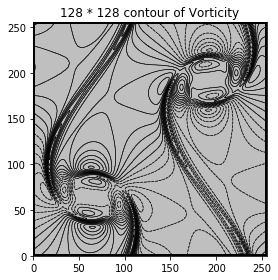
\includegraphics[width=0.5\textwidth]{figures/Voriticity_contour_128_128_c.png}
       \caption{Vorticity contour from the Minion and Brown's problem\cite{minion1997performance} setting  for resolution 128 $\times$ 128, number of contours being 20. Layer width parameter $\rho = 30$, viscosity $v=1/10,000$. }
       \label{fig:minion}
\end{figure}
In the parameters setting in Fig. 4 of Minion and Brown's work (seen Fig.~\ref{fig:minion}), there is a square system with a scale as $L_x = L_y = 1 unit = L$. The shear layer thickness $k$ they used is 30unit. Kinematic viscosity $\nu$ is $10^{-4}$. If we take $U = U_0 delta = 0.05$, $\nu$ = $10^{-4}$, and $L = 1$, then the corresponding Reynolds number is According to Equation~\ref{equ:neynolds}, we get the corresponding Reynolds number being 500, at Equation~\ref{Re_minion}:
\begin{equation}
\label{Re_minion}
    Re = UL / \nu = 0.05 x 1 / 10^{-4} = 500
\end{equation}

After calculate the Reynolds number of the Minion and Brown's work. We can adjust the initial parameters making the Reynolds the same in our implementation. Here, we set the simulation as $L_x = L_y = 128 = L$. The grid space is always $h = 1 unit$. The We now can apply the same initial velocities as Equation~\ref{equ:init_u_lbm}:

\begin{equation}
\label{equ:init_u_lbm}
    \begin{matrix}
u = U_0tanh(k (y-0.25L)) & y \leqslant 0.5 \\ 
u = U_0tanh(k (0.75L-y)) & y > 0.5  \\
v = \delta sin(2\pi x )
\end{matrix}
\end{equation}

Here, we should choose an equivalent value of shear layer thickness $k$; and, according to lattice Boltzmann method, the velocity unit $U_0$ should be less than the speed of sound $c_s$ and we choose $U_0 = 0.01$. To keep the Reynolds number the same, we can get the kinematic viscosity $\nu$ being 0.000128 by Equation~\ref{equ:nu_lbm}.

\begin{equation}
    \label{equ:nu_lbm}
    \nu = \frac{UL}{Re} = \frac{0.0005 \times 128}{500}  
\end{equation}

Finally, according to Minion and Brown's work, when T=0.8, there is a turbulence in the simulation; see Fig.~\ref{fig:minion}. We can calculate the time step (dimensionless time) by Equation\ref{timestep}. Substitute data from Minion and Brown's setting: time T = 0.8;  unit space $h=1/L=1/128$; unit velocity $U_0 \delta=U=0.05$  into the Equation\ref{timestep}, we know that in this system it need 2000 dimensionless time for the turbulence.

\begin{equation}
\label{timestep}
    T_{step} = \frac{T h}{U_0 \delta} = \frac{0.8 \times \frac{1}{128}}{0.005 } = 5.12
\end{equation}

In the lattice Boltzmann, we have unit space $h=1$, unit velocity $U_0 \delta = U = 0.0005$. Thus, substitute data into Equation~\ref{timestep}, we get $T_{step} = 2000 (timesteps)$, which means for every dimensionless time unit in Minion and Brown's system, we need 2000 steps to simulate to the same progress. In other words, to witness a turbulence in the lattice Boltzmann system, we need at least $5.12 \times 2000 = 10240$ steps. In the implementation and performance evaluation, we used 12000 steps as a standard; see Fig.~\ref{fig:minion}.\\

A more detailed initialization in serial C used for this project is at Appendix \ref{app:a}.


\vspace*{+3.2cm}
Having covered all the background material needed, we can now review the implementations that constitute one of the contributions of this project.

